\documentclass[11pt]{article}
\usepackage[a4paper,left=0.99in, right=0.99in,top=1.2in, bottom=1.2in]{geometry}

\usepackage[english]{babel}
\usepackage[a4paper]{geometry}
\usepackage{multicol}
\usepackage{graphicx}
\usepackage{amsfonts}
\usepackage{amsmath}
\usepackage{amssymb}
%\usepackage{breqn}
%\usepackage[]{fancyhdr}
\usepackage{tikz}
\usepackage{subcaption}
\usepackage{xcolor}
\usepackage{hyperref}
\usepackage{cite}
%\usepackage{ulem}

\usetikzlibrary{decorations}
\usetikzlibrary{snakes}

%-----------------------------------------------------------------------------
%\pagenumbering{arabic}
%\numberwithin{equation}{section}

%-----------------------------------------------------------------------------
\newcommand{\fww}[0]{\mathcal{F}^{\mathrm{WW}}}
\newcommand{\fdp}[0]{\mathcal{F}^{\mathrm{dipole}}}
\newcommand{\sdp}[0]{\sigma_{\mathrm{dipole}}}
\newcommand{\sdpa}[0]{\sigma_{\mathrm{dipole\,Adj.}}}
\newcommand{\GeV}[0]{\mathrm{GeV}}
\newcommand{\comment}[1]{\texttt{\color{red}#1}}
\newcommand{\commentPending}[1]{\texttt{\color{red!25}#1}}
\newcommand{\pairdot}[2]{ \mathbf{#1}\cdot\mathbf{#2}  }

%-----------------------------------------------------------------------------
\author{
T.~Goda,$^1$, K.~Kutak$^{1}$ and S.~Sapeta$^1$\\\,\\
$^1$ 
{\small\it The H.\ Niewodnicza\'nski Institute of Nuclear Physics PAN,}\\ 
{\small\it Radzikowskiego 152, 31-342 Krak\'ow, Poland}\\
}	 

\title{
Effects of gluon kinematics and the Sudakov\\
form factor on the dipole amplitude
}

\date{}

%-----------------------------------------------------------------------------
\begin{document}

\maketitle

%--------------- preprint numbers ---------------------
\vspace{-22em}
\begin{flushright}
  IFJPAN-IV-2023-XX
\end{flushright}
\vspace{17.5em}
%------------------------------------------------------

\begin{abstract}
We investigate effects of exact gluon kinematics on the parameters of the
Golec-Biernat--W\"usthoff, and Bartels--Golec-Biernat--Kowalski saturation
models. The resulting parameters show some differences, particularly, in the
normalization of the dipole cross section $\sigma_0$. The refitted models are
used for the dijet production process in DIS to investigate effects of the
Sudakov form factor at Electron Ion Collider energies.  
\end{abstract}

%%%%%%%%%%%%%%%%%%%%%%%%%%%%%%%%%%%%%%%%%%%%%%%%%%%%%%%%%%%%%%%%%%%%%%%%%%%%%%%%
\section{Introduction}

\comment{preprint number (SS)}\\
\comment{the information on energy and cuts is missing on the plots (KK)}
\comment{I reformulated some sentences added references and  interpretation of the curves where we use the KS gluon.  }


\begin{figure}[t]
\centering
\resizebox{0.6\textwidth}{0.2\textwidth}{
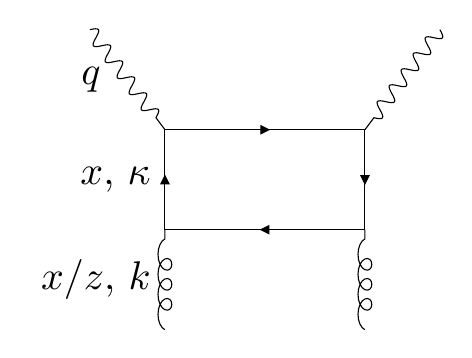
\begin{tikzpicture}
  \draw(-0.75in,0.25in)node[left,scale=0.02in]{$q$};
  \draw[snake=coil,segment aspect=0,segment length=0.1in](-0.875in , 0.5in)--(-0.5in,0.in);
  \draw[snake=coil,segment aspect=0,segment length=0.1in](0.875in ,0.5in)--(0.5in,0.in);
  \draw(-0.5in , 0in)--(0.5in,0in)--(0.5in , -0.5in)--(-0.5in,-0.5in)--cycle ;
  
  \filldraw(0.02in,0)--(-0.02in,-0.02in)--(-0.02in,0.02in)--cycle;
  \filldraw(-0.02in,-0.5in)--(0.02in,-0.52in)--(0.02in, -0.48in)--cycle;
  
  \filldraw(-0.5in,-0.23in)--(-0.52in,-0.27in)--(-0.48in,-0.27in)--cycle;
  \filldraw(0.5in,-0.27in)--(0.52in,-0.23in)--(0.48in,-0.23in)--cycle;
  
  \draw(-0.5in , -0.25in)node[left,scale=0.02in]{$x$, $\kappa$};
  \draw(-0.5in , -0.75in)node[left,scale=0.02in]{$x/z$, $k$};
  \draw[ snake=coil,segment aspect=1.5,segment length=0.1in](0.5in , -1in)--(0.5in,-0.5in);
  \draw[snake=coil,segment aspect=1.5,segment length=0.1in](-0.5in , -1in)--(-0.5in,-0.5in);
  \end{tikzpicture}
  \hspace{60pt}
  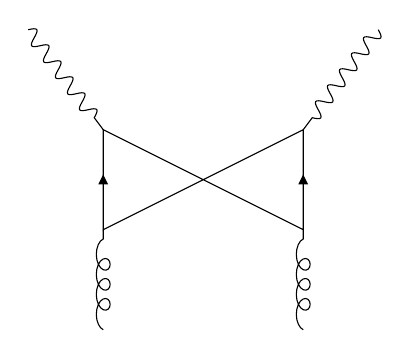
\begin{tikzpicture}
  \draw[snake=coil,segment aspect=0,segment length=0.1in](-0.875in , 0.5in)--(-0.5in,0.in);
  \draw[snake=coil,segment aspect=0,segment length=0.1in](0.875in ,0.5in)--(0.5in,0.in);
  \draw(-0.5in , 0in)--(0.5in,-0.5in)--(0.5in ,0in)--(-0.5in,-0.5in)--cycle ;
  
  \filldraw(-0.5in,-0.23in)--(-0.52in,-0.27in)--(-0.48in,-0.27in)--cycle;
  \filldraw(0.5in,-0.23in)--(0.52in,-0.27in)--(0.48in,-0.27in)--cycle;
  
  \draw[ snake=coil,segment aspect=1.5,segment length=0.1in](0.5in , -1in)--(0.5in,-0.5in);
  \draw[snake=coil,segment aspect=1.5,segment length=0.1in](-0.5in , -1in)--(-0.5in,-0.5in);
\end{tikzpicture}
}
\caption{Kinematic variables of the inclusive DIS. \commentPending{Photon momentum (TG)}}
\label{fig:gluon-kinem}
\end{figure}

Factorization of scales plays central role in {\it Quantum Chromodynamics}
(QCD). In particular, within collinear factorization approach, long-distance
effects can be isolated into objects called {\it collinear parton distribution
functions}~(PDFs)~\cite{Roberts:1990ww,Collins:2011zzd}.  The collinear PDFs are
not fully perturbatively calculable but they obey perturbative evolution
equations and are process independent~\cite{Collins:2011zzd}. That is to say
that one needs to measure them in experiments, but the PDFs obtained in one
experiment can be used as input in another. 

One of the main type of processes that is suited particularly well to the
studies of proton structure is the {\it deep inelastic
scattering}~(DIS)~\cite{Roberts:1990ww,Collins:2011zzd}. The data from HERA has
enabled us to answer many questions in that domain and largely improved our
picture of interior of a proton.  It is therefore very exiting that the next
generation of a DIS machines, the Election Ion Collider~(EIC)~\cite{NAP25171} is
making its way and will soon allow us to uncover more details about the hadron
structure.

At large center of mass energy and fixed value of the photon virtuality, $Q$,
one probes  the region of small Bjorken scaling variable, $x$.  In that region,
dominated by gluons\cite{Roberts:1990ww,Collins:2011zzd, Kovchegov:2012mbw}, the
approach of High Energy Factorization, also called
$k_T$-factorization~\cite{Catani:1990xk,Catani:1990eg,Collins:1991ty,Catani:1993ww,Catani:1993rn,Catani:1994sq},
has proven to be suited particularly well.  In this framework, the interaction
of the photon with gluons happens through a box of quarks, as depicted in
Fig.~\ref{fig:gluon-kinem}. An object, which is central to the description of
this process is called the dipole gluon density, $\fdp(x,k_T^2)$, which is a
type of {\it transverse momentum dependent} PDFs (TMD
PDFs)~\cite{Bomhof:2006dp,Dominguez:2010xd,Dominguez:2011wm,Xiao:2017yya}. 
%
Due to its clear picture, one often uses a position-space counterpart of the gluon density, called {\it dipole cross section}. 
%
It appears in the $k_T$-factorization
formula~\cite{Catani:1990eg,Dominguez:2010xd,Dominguez:2011wm,Xiao:2017yya},
which we shall discuss in the next section, and plays a role similar to that of
the collinear parton distribution function in the collinear factorization.  

Much effort has been made to study this object, notably the work of Balitsky,
Fadin, Kuraev and Lipatov (BFKL)~\cite{Balitsky:1978ic, Kuraev:1977fs} has
predicted sharp rise of cross sections with $1/x$.  However, such rise violates
unitarity and the Froissart
bound~\cite{Roberts:1990ww,Collins:2011zzd,Kovchegov:2012mbw,Barone:1993sy}. In
Ref.~\cite{Gribov:1983ivg} it has been recognized that gluon recombination can
tame the growth of gluons. The interplay of linear and
nonlinear terms leads to a phenomenon called {\it gluon saturation} and
corresponding evolution equations are known as
Balitsky-Kovchegov~(BK)~\cite{Balitsky:1995ub,Kovchegov:1999yj} equation or
JIMWLK\cite{Kovner:1999bj,Kovner:2000pt,Iancu:2000hn,JalilianMarian:1997dw,JalilianMarian:1997gr,JalilianMarian:1997jx}
equation.

Despite the success of the aforementioned evolution equations, there exist a
number of phenomenological models of the dipole cross section, which are popular
due to to their simplicity.  A notable example is the model proposed by
Golec-Biernat and Wu\"sthoff (GBW)~\cite{Golec-Biernat:1998zce} and its
extension by Bartels, Golec-Biernat and Kowalski (BGK)~\cite{Bartels:2002cj}. We
will use these two specific models in our study. We note, however, that other
saturation models have been discussed in the
literature~\cite{Kowalski:2003hm,McLerran:1993ni,Forshaw:1999uf,Iancu:2003ge}.

In the present study, we fit the GBW and BGK models to HERA
data~\cite{Abt:2017nkc} in the $k_T$-factorization formula of $F_2$, instead of
the original dipole factorization formula. As discussed below, this allows us to relatively easy investigate the role 
of the  exact gluon kinematics.  Since inclusive observables do not
reveal the $k_T$ dependence well, in order to demonstrate the effects of exact kinematics we consider a less inclusive observable
which is more sensitive to the $k_T$ dependence of the gluon distribution.  The
resulting models are used for predictions of dijet production in DIS at EIC,
including effects of the Sudakov form factor, which resums logarithms of the
small transverse momentum. 
%
This process is known to be sensitive to another type of gluon density, called
Weitzs\"acker-Williams~\cite{Dominguez:2010xd,Dominguez:2011wm}. For that
process, we study, in particular, the angular correlation of jets, and that of
the scattered electron and the jets.
 
The paper is organized as follows.  In the next section, we present theoretical
framework which we use and outline differences between the $k_T$-factorization
and the dipole factorization.  In Sec.~\ref{sec:F2fits}, results of the new fits
to HERA data in the $k_T$-factorization formula are presented.  In
Sec.~\ref{sec:dijetsEIC}, we apply the results from the previous section to
compute distributions for dijet production in DIS at the EIC and make
comparisons to our earlier study of Ref.~\cite{vanHameren:2021sqc}.

%%%%%%%%%%%%%%%%%%%%%%%%%%%%%%%%%%%%%%%%%%%%%%%%%%%%%%%%%%%%%%%%%%%%%%%%%%%%%%%%
\section{The framework}
%%%%%%%%%%%%%%%%%%%%%%%%%%%%%%%%%%%%%%%%%%%%%%%%%%%%%%%%%%%%%%%%%%%%%%%%%%%%%%%%

The DIS cross section (structure function) factorises and can be written in a
form
%
\begin{equation}
   d\sigma = \sum_{a}  \phi_{a/h} \otimes H_{\gamma a \to X} ,
\end{equation}
%
where the hard function, $H_{\gamma a \to X}$, involving a parton $a$ in the
initial state, is calculable perturbatively, and $\phi_{a/h}$ is the parton
distribution function of $a$ in a hadron $h$.  
%
The symbol $\otimes$ denotes appropriate convolution. All nonperturbative
effects are absorbed in $\phi_{a/h}$, while $H_{\gamma a \to X}$ can be computed
order by order in $\alpha_s$.  
 
We will study factorization in two versions: defined in momentum and position
space respectively.  As mentioned earlier, in the fit we use the GBW and BGK models.  The models were
originally formulated in the position-space version of the $k_T$-factorization
formula.  In the GBW model, the dipole cross section has the
form~\cite{Golec-Biernat:1998zce}
%
\begin{align}
\label{eq:gbw-dipole}
\sigma_{\mathrm{GBW}}(x,r)&=\sigma_0\left(1-e^{-r^2/R^2_0}\right)&\mathrm{where}&
&R^{-2}_0&=\frac{Q_0^{2}}{4}\left(\frac{x_0}{x}\right)^\lambda.
\end{align}
%
The dipole cross section is related to the dipole gluon density by the Fourier
transform
%
\begin{equation}
\alpha_s\fdp(x,k_T^2)=\frac{N_c}{4\pi}\int\frac{d^2\mathbf{r}}{(2\pi)^2}e^{i\mathbf{k}_t\cdot \mathbf{r} }\nabla_{\mathbf{r}}^2\sigma_{\mathrm{dipole}}(x,r).
\label{eq:dipole gluon}
\end{equation}
%
The essence of the GBW model is encoded in the $x$-dependent saturation scale
$Q_s^2(x)=Q^2_0(x_0/x)^{-\lambda}$, which separates the saturation region and
the scaling region.  An extension of the above model was proposed by Bartels, Golec-Biernat
and Kowalski~\cite{Bartels:2002cj} who incorporated the DGLAP evolution
in the GBW dipole cross section~(\ref{eq:gbw-dipole}) by modifying the exponent
to 
%
\begin{equation}
R_0^{-2}=\frac{\pi^2\alpha(\mu^2)xg(x,\mu^2)}{3\sigma_0},
\end{equation}
where
\begin{align}
\mu^2&=\frac{C}{r^2}+\mu_0^2 & &\mathrm{and} & xg(x,Q^2_0)&=A_g x^{-\lambda_g}(1-x)^{5.6},
\end{align}
%
thus improving the description of data at higher $Q^2$.\\

While these models enjoyed much success in phenomenology of DIS, including the
diffractive and photo-production
processes~\cite{Golec-Biernat:1998zce,Golec-Biernat:1999qor}, it is worth
mentioning that they both use certain kinematic approximation which follows from
subtle differences in the dipole factorization and the $k_T$-factorization.  In
the following, we will investigate effects of these approximations.

Firstly, let us outline the factorization formulas.
With $q'\equiv q+x p$, one decomposes $k$ and $\kappa$, defined in
Fig.~\ref{fig:gluon-kinem}, as
%
\begin{align}
    \kappa&=\alpha p-\beta q'+\kappa_t&&\mathrm{and}& k&=a p- bq'+k_T.
\end{align}
%
For the contribution depicted in Fig.~\ref{fig:gluon-kinem}, the structure
function $F_2$ factorizes with a change of variable
${\boldsymbol{\kappa}'}_t\equiv{\boldsymbol{\kappa}_t}-(1-\beta)\mathbf{k}_t$,
to the form~\cite{ Kimber:2001uaa,Kwiecinski:1997ee}
%
\begin{multline}
	F_2(x,Q^2)=\sum_f e_f^2 \frac{Q^2}{2\pi}\int\frac{dk^2_t}{k_T^2}\int^1_0d\beta\int d{\kappa'}_t\alpha_s(\mu^2) \fdp(x/z,k_T^2)\Theta(1-x/z)\\
	\left[\left(\beta^2+(1-\beta)^2\right)\left(\frac{I_1}{2\pi}-\frac{I_2}{2\pi}\right)
	+\left(m_f^2+4Q^2\beta^2(1-\beta)^2\right)\left(\frac{I_3}{2\pi}-\frac{I_4}{2\pi}\right)\right],
	\label{eq:angle-integrated}
\end{multline}
where
\begin{equation}
	\frac{1}{z}=1+\frac{{\kappa'}^2_t+m_f^2}{\beta(1-\beta)Q^2}+\frac{k^2_t}{Q^2}\,.
	\label{eq:z}
\end{equation}

One should note that the gluons are not probed directly, thus the argument of
the gluon density is $x/z$ rather than $x$.  If one, instead, uses $ 1/z=1+4
m_f^2/Q^2$ and assumes that $\mu$ is independent of $\kappa'$ and $k_T$, the
above formula can be written in the impact parameter
space~\cite{Golec-Biernat:1998zce,Nikolaev:1990ja} ({\it i.e.} as a dipole
factorization formula)
%
\begin{equation}
  F_2\left(x,Q^2\right)=\sum_f e_f^2 \frac{Q^2}{4\pi^2} \int^1_0d\beta \int \frac{d^2\mathbf{r}}{(2\pi)^2} \left|\Psi\left(\tilde{x},\beta,Q^2\right)\right|^2\sigma_{\mathrm{dipole}}\left(\tilde{x},r\right),
  \label{eq:dipole factorization}
\end{equation}
%
where the photon wave function, $\left|\Psi\left(x,\beta,Q^2\right)\right|^2$,
describes splitting of the incoming photon into a $q\overline{q}$ pair with
light-cone momenta fractions $\beta$ and $1-\beta$ respectively, and the dipole
cross section, $\sigma_{\mathrm{dipole}}\left(\tilde x,r\right)$, describes the
interaction of the colour dipole of size $r$ with the proton. In
Ref.~\cite{Golec-Biernat:1998zce}, $\tilde{x}=x(1+4m_f/Q^2)$ with nonzero value
of $m_f$ was used even for light flavours, which is necessary to partially
substitute $k_T$ and ${\kappa'}_T$ in Eq.~(\ref{eq:z}).
%The original GBW and BGK models were fitted in the dipole factorization, Eq.~(\ref{eq:dipole factorization}), while 
In the present study, we use Eq.~(\ref{eq:angle-integrated}) to fit the models, where the gluon density is obtained by evaluating Eq.~(\ref{eq:dipole gluon}).
%Comparing, the GBW and BGK models, one identifies that, the GBW model is effectively the BGK model with 
%\begin{equation}
%\begin{split}
%    \alpha_s(\mu^2)xg(x,\mu^2)\rightarrow &\alpha_s(Q_0^2)xg(x,Q_0^2)\\
%    &=\alpha_s x^{-\lambda}(1-x)^{5.6}.
%\end{split}
%\end{equation}

Considering the small-$r$ limit of the GBW model, 
\begin{equation}
    \left.\sigma_{\mathrm{GBW}}\left(x,r\right)\right|_{r\ll Q_s}\approx r^2
    Q_s^2/4\,,
\end{equation}
comparison to 
\begin{equation}
\left. \sigma_{\mathrm{dipole}}\left(x,r\right)\right|_{r\ll
Q_s}\approx\frac{r^2 \pi^2\alpha_s(\mu^2)xg(x,\mu^2)}{3}\,,
\end{equation} 
%
from BGK, suggests that the GBW model is an approximation in which
$\alpha_s(\mu^2)$ and $xg(x,\mu^2)$ are independent of
$r$~\cite{Bartels:2002cj}.  
%
For this reason, in one version of the model discussed below, we shall account
for the running coupling in Eq.~(\ref{eq:angle-integrated}), by assuming that
$\alpha_s$ in Eq.~(\ref{eq:dipole gluon}) is constant for the GBW model, and
thus explicitly multiply it by the running coupling
%
\begin{equation}
\alpha_s(\mu^2)\fdp(x,k_T^2)\rightarrow \alpha_s(\mu)\frac{\alpha_s\fdp(x,k_T^2)}{0.2},
\end{equation}
where
%
\begin{equation}
\alpha_s(\mu^2)=\frac{1}{\frac{11 C_A-2n_f}{12\pi}\log\left(\frac{\mu^2}{\Lambda_{\mathrm{QCD}}^2 }\right)},
\end{equation}
and  $\Lambda_{\mathrm{QCD}}^2=0.09\;\GeV^2$.

The factor 0.2 is an arbitrary normalization, whose effect is absorbed by
$\sigma_0$, and hence bears no importance.  (For a more detailed analysis of the
dipole gluon density from the BGK model see
Ref.~\cite{Luszczak:2022fkf}\footnote{In Ref.~\cite{Luszczak:2022fkf}, the
coupling constant was treated differently, and the large $k_T$-region was
matched to the derivative of $xg(x)$, while we have used series transformation
to accelerate the high-$k_T$ integration. Their treatment is also different from
the original BGK paper~\cite{Bartels:2002cj}. As a consequence their gluon
density is positive in the large $k_T$-region and the overall large-$k_T$
behaviour is significantly different.}) While there is some ambiguity on what
the argument of $\alpha_s(\mu^2)$ should be, we follow
Ref.~\cite{Kwiecinski:1997ee} and use
%
\begin{equation}
	\mu^2=k_T^2+{\kappa'}_t^2+m_f^2+\mu^2_0,
\end{equation}
%
where we add $\mu^2_0=4\;\GeV^2$ in order to freeze the coupling at low scales.

%%%%%%%%%%%%%%%%%%%%%%%%%%%%%%%%%%%%%%%%%%%%%%%%%%%%%%%%%%%%%%%%%%%%%%%%%%%%%%%%
\section{Fits to $F_2$ data}
\label{sec:F2fits}

We fitted the GBW and BGK models to the $F_2$ data from
HERA~\cite{Abt:2017nkc}. A numerical program was written with help of
CERNLIB~(DPSIPG)~\cite{Kolbig:1972zz}, GSL~\cite{GSL}, CUBA~\cite{Hahn:2004fe}
and ROOT~\cite{Brun:1997pa} libraries to evaluate $F_2$. The fitting was
performed using MnMigrad and MnSimplex of ROOT::Minuit2~\cite{James:2004xla}.

The data were selected to be in the range $0.045\leq Q^2\leq
650\;\mathrm{GeV^2}$, $x<0.01$.  As with the previous fit~\cite{Goda:2022wsc},
the $c$ and $b$ flavours were taken into account with the mass $1.3$ and
$4.6\;\mathrm{GeV}$, respectively. As discussed earlier, we take the light
quarks to be massless.  

We studied the following cases
%
\begin{itemize}
\item GBW model with the fixed coupling in $k_T$-factorization  ($k_T$-GBW),
\item GBW model with the running coupling in $k_T$-factorization (rc-$k_T$-GBW),
\item BGK model in $k_T$-factorization ($k_T$-BGK),
\end{itemize} 
%
and, as a reference, we provide the following results from
Ref.~\cite{Goda:2022wsc};
%
\begin{itemize}
\item GBW model with massless light quarks in the dipole factorization ($r$-GBW),
\item GBW model with massive light quarks in the dipole factorization ($r$-GBW-massive),
\item  BGK model in  the dipole factorization ($r$-BGK).
\end{itemize} 

%-----------------------------------------------------------------------------
\begin{table}[t]
\begin{subtable}{\textwidth}
\center\footnotesize
\begin{tabular}{|c|c|c|c|c|}
	\hline - & $\sigma_0 $ [mb] & $x_0 \left(10^{-4}\right)$ & $\lambda$ & $\chi^2/\mathrm{dof}$ \\\hline 
	{\footnotesize $r$-GBW} & 1.907e+01& 2.582e+00& 3.219e-01& 4.438e+00\\\hline 
	{\footnotesize $r$-GBW-massive} & 2.384e+01& 1.117e+00& 3.082e-01& 5.274e+00\\\hline 
	{\footnotesize $k_t$-GBW} & 3.344e+01& 1.333e+00& 3.258e-01& 4.396e+00\\\hline 
	{\footnotesize rc-$k_t$-GBW} & 1.520e+01& 2.648e+00& 3.211e-01& 2.447e+00\\\hline 
\end{tabular}
%\caption{}
\vspace{2mm}
\end{subtable}
\begin{subtable}{\textwidth}
\center\footnotesize
\begin{tabular}{|c|c|c|c|c|c|c|}
	\hline - & $\sigma_0 $ [mb] & $A_g$ & $\lambda_g$ & $C$ & $\mu_0^2 \left[\mathrm{GeV^2}\right]$ & $\chi^2/\mathrm{dof}$ \\\hline 
	{\footnotesize $r$-BGK} & 2.326e+01& 1.181e+00& 8.317e-02& 3.294e-01& 1.873e+00& 1.556e+00\\\hline 
	{\footnotesize $k_t$-BGK} & 3.470e+01& 1.048e+00& 2.205e-01&2.391e-01& 9.954e-01&  1.527e+00\\\hline 
\end{tabular}
%\caption{}
\vspace{2mm}
\end{subtable}
\caption{Fit parameters of respective models. The parameters of the
dipole factorization cases are from Ref.~\cite{Goda:2022wsc}.}
\label{tab:table}
\end{table}
%-----------------------------------------------------------------------------

The results of the fits are summarized in Tab.~\ref{tab:table}. 
The fit quality of $k_T$-GBW is almost unchanged w.r.t. $r$-GBW, while rc-$k_T$-GBW shows remarkable improvement, almost halving the $\chi^2$ value.
This is in line with the observation made in Refs.~\cite{Albacete:2004gw,Albacete:2007yr,Albacete:2010sy} that in the BK evolution, the running coupling correction have considerable effects.

Another notable point is that, except for the normalization $\sigma_0$, the parameters are very similar, particularly those of rc-$k_T$-GBW are almost identical to those of $r$-GBW. 
While the GBW model remains almost unaffected, the BGK model seems to show slightly more change. The difference in $\sigma_0$ is similar to that of GBW model, and other parameters changed moderately.

In Fig.~\ref{fig:GBW-BGK}, the plots of the dipole cross section, the dipole
gluon density and the saturation scale for the GBW and BGK models are shown. The
dipole cross section and the gluon density are both normalized by $\sigma_0$ in
order to see the effects  of other parameters better, and the saturation scale
is defined as a ridge of the dipole gluon density in the $(x,k_T^2)$ plane.

In the plots on the left side, one can see the effects of the changes in the
parameters of the GBW model. The difference between the rc-$k_T$-GBW and $r$-GBW
is negligible, while the $k_T$-GBW is slightly shifted, compared to others, by the change in $x_0$.

On th right side of Fig.~\ref{fig:GBW-BGK}, the same plots are shown for the BGK
model. Unlike in the GBW case, the connection between the differences shown in
the plots and the differences in the parameters is less clear. Nevertheless, the
difference is more prominent in the small-$x$ region.

Comparisons of the results with the $F_2$ data are shown in
Figs.~\ref{fig:GBW-Grid} and~\ref{fig:BGK-Grid}.  In Fig.~\ref{fig:GBW-Grid},
the differences between $r$-GBW and $k_T$-GBW are not visible, while
rc-$k_T$-GBW shows sizable difference from the others, particularly in the
large-$Q^2$ region.  Recalling that the parameters of rc-$k_T$-GBW and $r$-GBW
are very similar, the difference in $F_2$ is almost entirely due to the coupling
constant. The improvement in the fit quality is depicted as a histogram of the
$\chi^2$-vale per number of points at the bottom of Fig.~\ref{fig:GBW-Grid}.
Here, the improvement in the large-$Q^2$ region is very clear.  In
Fig.~\ref{fig:BGK-Grid}, the difference between $r$-BGK and $k_T$-BGK are hardly
visible. In the histogram at the bottom, one can see some differences, but they
cancel out mostly, making little improvement overall.

\begin{figure}[p]

  \begin{multicols}{2}
  \begin{subfigure}{0.5\textwidth}
    \includegraphics[width=\textwidth]{./plots/GBW-dipole.pdf}
    \includegraphics[width=\textwidth]{./plots/GBW-gluon.pdf}
    \includegraphics[width=\textwidth]{./plots/GBW-saturation.pdf}
    \caption{GBW}
    \label{fig:GBW}
\end{subfigure}
\begin{subfigure}{0.5\textwidth}
    \includegraphics[width=\textwidth]{./plots/BGK-dipole.pdf}
    \includegraphics[width=\textwidth]{./plots/BGK-gluon.pdf}
    \includegraphics[width=\textwidth]{./plots/BGK-saturation.pdf}
    \caption{BGK}
    \label{fig:BGK}
\end{subfigure}
  \end{multicols}
  \caption{The dipole cross section, the dipole gluon density at $x=10^{-2},\;
  10^{-6}$, and the saturation scale for the GBW (left) and the BGK (right)
  models. Note that the dipole cross section and the gluon density are
  normalized with $\sigma_0^{-1}$.} 
\label{fig:GBW-BGK}
\end{figure}

\begin{figure}[p]
%\begin{subfigure}{\textwidth}
\includegraphics[width=0.49\textwidth]{./plots/Figure_1.png}
\includegraphics[width=0.49\textwidth]{./plots/Figure_2.png}
\includegraphics[width=\textwidth]{./plots/Figure_3.png}
%\end{subfigure}
\caption{Comparison of $F_2$ fro GBW with HERA data. The histogram shows the
$\chi^2$ value per data point in each frame.  Improvement by the running
coupling (rc-$k_T$) is clearly visible in the high-$Q^2$region, while the new
fit ($k_T$) shows only marginal improvement.}
\label{fig:GBW-Grid}
\end{figure}

\begin{figure}[p]
%\begin{subfigure}{\textwidth}
\includegraphics[width=0.49\textwidth]{./plots/Figure_2-1.png}
\includegraphics[width=0.49\textwidth]{./plots/Figure_2-2.png}
\includegraphics[width=\textwidth]{./plots/Figure_2-3.png}
%\end{subfigure}
\caption{Comparison of $F_2$ from BGK with HERA data. The histogram shows the
$\chi^2$ value per data point in each frame. The overall fit quality
remain similar but the quality in each frame changes noticeably. In
particularly, the $k_T$-formula ($k_T$) shows better quality at small $Q^2$.}
\label{fig:BGK-Grid}
\end{figure}

Let us now take a closer look at the parameter $\sigma_0$. Recall that the
difference between the $k_T$-factorization formula and the dipole factorization
formula is in $x/z$, and this enters in the GBW formalism as
$\tilde{x}$. It is easy to see that, as $x$ grows, the dipole cross section gets
suppressed. (Keeping in mind the suppression by the photon wave function in the
large-$r$ region.) Such effect was discussed previously in
Ref.~\cite{Kutak:2004ym} in the context of the BK equation. In fact, this
suppression is the motivation given in Ref.~\cite{Golec-Biernat:1998zce} for
such modification of $x$, so that in the small-$Q^2$ limit, the total cross
section remains finite. Since 
%
\begin{equation}
\left(1+\frac{4 m_f^2}{Q^2}\right)\leq\left(1+\frac{k_T^2}{Q^2}+\frac{{\kappa'}_t^2+m_f^2}{\beta(1-\beta)Q^2}\right),
\end{equation}
%
the $k_T$-factorization case receives more suppression. Consequently, the
normalization factor $\sigma_0$ rises to compensate the suppression.  Therefore,
one can understand the change in $\sigma_0$ as a direct consequence of the key
difference between the $k_T$-factorization and the dipole factorization.

%%%%%%%%%%%%%%%%%%%%%%%%%%%%%%%%%%%%%%%%%%%%%%%%%%%%%%%%%%%%%%%%%%%%%%%%%%%%%%%%
\section{Dijet production at EIC}
\label{sec:dijetsEIC}

\begin{figure}[t]
    \begin{subfigure}{0.5\textwidth}
        \includegraphics[width=\textwidth]{plots/GBWWW1} 
    \end{subfigure}
    \begin{subfigure}{0.5\textwidth}
        \includegraphics[width=\textwidth]{plots/BGKWW1} 
    \end{subfigure}
    \begin{subfigure}{0.5\textwidth}
        \includegraphics[width=\textwidth]{plots/GBWWW2} 
    \end{subfigure}
    \begin{subfigure}{0.5\textwidth}
        \includegraphics[width=\textwidth]{plots/BGKWW2} 
    \end{subfigure}
    \caption{ Weizs\"acker-Williams gluon density at $x=10^{-3}$. Top row:
    comparison of the dipole factorization fit and $k_T$-factorization fit
    results. Bottom row: comparison of the respective models with and without
    the Sudakov factor, at $\mu=17,\;67\ \mathrm{GeV}$.The green dotted line is the KS gluon~\cite{vanHameren:2021sqc}, and the green dashed line is the rcBK gluon~\cite{Hentschinski:2022rsa}. }
    \label{fig:ww}
\end{figure}

\begin{figure}[p]
	\begin{subfigure}{0.5\textwidth}
	\includegraphics[width=\textwidth]{plots/plotGBW1} 
	\end{subfigure}
	\begin{subfigure}{0.5\textwidth}
	\includegraphics[width=\textwidth]{plots/plotBGK1} 
	\end{subfigure}
	\begin{subfigure}{0.5\textwidth}
	\includegraphics[width=\textwidth]{plots/plotGBW2}
	\end{subfigure}
	\begin{subfigure}{0.5\textwidth}
	\includegraphics[width=\textwidth]{plots/plotGBW3}
	\end{subfigure}
	\begin{subfigure}{0.5\textwidth}
	\includegraphics[width=\textwidth]{plots/plotBGK2}
	\end{subfigure}
	\begin{subfigure}{0.5\textwidth}
	\includegraphics[width=\textwidth]{plots/plotBGK3}
	\end{subfigure}
	\caption{ Azimuthal correlation of the jets and the scattered electron in the Breit frame. Top: Comparison of dipole factorization fit and $k_T$-factorization fit. Middle \& Bottom: Effect of the Sudakov form factor. The green dotted line is the KS gluon~\cite{vanHameren:2021sqc}, and the green dashed line is the rcBK gluon~\cite{Hentschinski:2022rsa}.}
	\label{fig:je-breit}
\end{figure}

\begin{figure}[p]
	\begin{subfigure}{0.5\textwidth}
		\includegraphics[width=\textwidth]{plots/plotGBW1Lab} 
	\end{subfigure}
	\begin{subfigure}{0.5\textwidth}
		\includegraphics[width=\textwidth]{plots/plotBGK1Lab} 
	\end{subfigure}

	\begin{subfigure}{0.5\textwidth}
		\includegraphics[width=\textwidth]{plots/plotGBW2Lab}
	\end{subfigure}
	\begin{subfigure}{0.5\textwidth}
		\includegraphics[width=\textwidth]{plots/plotGBW3Lab}
	\end{subfigure}

	\begin{subfigure}{0.5\textwidth}
		\includegraphics[width=\textwidth]{plots/plotBGK2Lab}
	\end{subfigure}
	\begin{subfigure}{0.5\textwidth}
		\includegraphics[width=\textwidth]{plots/plotBGK3Lab}
	\end{subfigure}
\caption{ Azimuthal correlation of the jets and the scattered electron in the lab frame. Top: Comparison of dipole factorization fit and $k_T$-factorization fit. Middle \& Bottom: Effect of the Sudakov form factor. The green dotted line is the KS gluon~\cite{vanHameren:2021sqc}, and the green dashed line is the rcBK gluon~\cite{Hentschinski:2022rsa}.}
\label{fig:je-lab}
\end{figure}

\begin{figure}[p]
	\begin{subfigure}{0.5\textwidth}
		\includegraphics[width=\textwidth]{plots/plotGBW1Jets} 
	\end{subfigure}
	\begin{subfigure}{0.5\textwidth}
		\includegraphics[width=\textwidth]{plots/plotBGK1Jets} 
	\end{subfigure}

	\begin{subfigure}{0.5\textwidth}
		\includegraphics[width=\textwidth]{plots/plotGBW2Jets}
	\end{subfigure}
	\begin{subfigure}{0.5\textwidth}
		\includegraphics[width=\textwidth]{plots/plotGBW3Jets}
	\end{subfigure}

	\begin{subfigure}{0.5\textwidth}
		\includegraphics[width=\textwidth]{plots/plotBGK2Jets}
	\end{subfigure}
	\begin{subfigure}{0.5\textwidth}
		\includegraphics[width=\textwidth]{plots/plotBGK3Jets}
	\end{subfigure}
\caption{Azimuthal correlation of the jets in the Breit frame. Top: Comparison of dipole factorization fit and $k_T$-factorization fit. Middle \& Bottom: Effect of the Sudakov form factor. The green dotted line is the KS gluon~\cite{vanHameren:2021sqc}, and the green dashed line is the rcBK gluon~\cite{Hentschinski:2022rsa}. }
\label{fig:jj-breit}
\end{figure}




The $F_2$ structure function is an inclusive object and it is weakly sensitive
to the shape of the gluon density. To probe the shape better, we shall now apply the
dipole cross sections obtained in the previous section to the electron-dijet
correlation at EIC, following closely the method of Ref.~\cite{vanHameren:2021sqc}.  

We consider dijet production in DIS
%
\begin{equation}
  %\label{eq:}
  e+p\rightarrow e+J_1+J_2+X\,.
\end{equation}
%
At the leading order, in the small-$x$ limit, this process is
dominated by $q\overline{q}$ jets~\cite{Dominguez:2011wm}.  It is
therefore closely related to the dipole picture we discussed earlier. In the Breit frame, where the photon momentum is
given by $q=(0,0,0,Q)$, at the leading order, the jets momentum imbalance
$p_T\equiv\left|p_{1T}+p_{2T}\right|$ equals the gluon transverse momentum
$k_T$, where $p_{1T}$ and $p_{2T}$ are transverse momenta of the jets.  This
makes dijets an interesting process. For the region where $p_T\ll P_T\sim
p_{1T},\,p_{2T}$, one may use power counting to take leading order in $p_T/P_T$,
which leads to the transverse-momentum-dependent~(TMD) factorization.
  
In the large-$N_c$ limit of the TMD factorization, there are two types of gluon
densities, namely the dipole gluon density and the Weizs\"acker-Williams (WW)
gluon
density~\cite{Dominguez:2010xd,Dominguez:2011wm,vanHameren:2016ftb,Xiao:2017ggh}.
It was shown in Ref.~\cite{Dominguez:2011wm}, that the dijet process in DIS can
directly probe the WW gluon, $\fww(x,k^2)$, where the differential cross section
factorizes as
%
\begin{equation}
	\frac{d\sigma^{\gamma^*p\rightarrow q\overline{q}X}}{d \mathrm{P.S.}}=\fww(x,k_T^2)H_{\gamma^*g^*\rightarrow q\overline{q}},
        \label{eq:TMD}
\end{equation}
%
with the hard function $H_{\gamma^*g^*\rightarrow q\overline{q}}$ describing
interactions of an off-shell photon with an off-shell gluon producing a
$q\overline{q}$ pair.  $\fww(x,k^2)$, has an interpretation as a number density
of gluons inside a proton, while $\fdp(x,k_T^2)$ does not have such an
interpretation~\cite{Dominguez:2010xd,Dominguez:2011wm,Xiao:2017ggh}.  

We carry out our study in the framework of the {\it Improved
Transverse-Momentum-Dependent} (ITMD)
factorization~\cite{Kotko:2015ura,vanHameren:2016ftb}.  This is
implemented in the program KaTie~\cite{vanHameren:2016kkz}, which we use to
compute the cross sections.  The ITMD factorization is a generalization of the
TMD factorization, where the momentum imbalance in TMD is restricted to be
small~\cite{Kotko:2015ura,vanHameren:2016ftb}. That is to say, ITMD resums
$(Q_s/k_T)^n$ and $(k_T/P_T)^n$~\cite{Kotko:2015ura,vanHameren:2016ftb}, thus
extends the region of applicability up to $k_T\sim P_T$. The difference of
Eq.~(\ref{eq:TMD}) from the regular TMD is that the hard function has an
off-shell gluon, $g^*$, thus rendering the $k_T$ dependence in the hard function
as well~\cite{Kotko:2015ura}.

Under the Gaussian approximation and assuming $\theta$-like profile of the
proton, one can
write~\cite{vanHameren:2016ftb,Xiao:2017ggh,Dominguez:2010xd,Dominguez:2011wm}
%
\begin{equation}
\fww(x,k^2)= \frac{C_F}{2\pi^3\alpha_s}\int^\infty_0\frac{dr}{r}J_0(r k) \sdpa(x,r),
\end{equation} 	
with the adjoint dipole cross section
\begin{equation}
\sdpa(x,r)=\sigma_0\left( 1-\left(1-\frac{\sdp(x,r)}{\sigma_0}\right)^{C_A/C_F}\right).
\label{eq:ww}
\end{equation}

For the region where TMD factorization is applicable, $Q_s\sim k_T\ll P_T\sim
Q$, one needs to resum the large Sudakov logarithms $\log(k_T/Q)$, as well as
$\log(1/x)$~\cite{Dominguez:2011wm}. It was shown in
Refs.~\cite{Mueller:2012uf,Mueller:2013wwa,Xiao:2017yya} that consistent
resummation of such logarithms is possible owing to the separation of
corresponding regions.  Resummation of the Sudakov logarithms is achieved by the
formula
%
\begin{equation}
	\fww(x,k^2,\mu^2)= \frac{C_F}{2\pi^3\alpha_s}\int^\infty_0\frac{dr}{r}J_0(r k) e^{-S(r,\mu^2)} \sdpa(x,r),
	\label{eq:ww-sud}
\end{equation}
%
where, we use the Sudakov form factor~\cite{Mueller:2013wwa,Xiao:2017yya},
%
\begin{equation}
	S(r,\mu^2)=\frac{\alpha_s N_c}{4\pi}\ln^2\left(\frac{\mu^2r^2}{4e^{-2\gamma_E}}\right),
\end{equation}
%
in which $\gamma_E$ is the Euler-Mascheroni constant, and we set $\alpha_s=0.2$. 
Following Ref.~\cite{vanHameren:2021sqc}, we study the azimuthal correlations of
jets and the final state electron in DIS , where
it was argued that this observable is sensitive to the soft emissions and the
saturation effects. In this study we focus only on the proton case.  The
kinematical cuts suggested in Ref.~\cite{vanHameren:2021sqc} were
%
\begin{align*}
	E_e&=15\GeV& E_p&=135\GeV& Q^2&>1\GeV^2\\
	0.1<&\nu<0.85&\Delta R_{\mathrm{Breit}}&<1&p^{\mathrm{Breit}}_{1,2\,T}&>3\GeV\\
	&&-4<&y_{1,2\,\mathrm{lab}}<-1.&&
\end{align*}

\comment{Normalization (SS) Comment in context of Figs. 6, 7, 8 (TG)}

\comment{Another rcBK (TG)}


Grids of the Weizs\"acker-Williams gluon density were produced by evaluating
Eqs.~(\ref{eq:ww}) and~(\ref{eq:ww-sud}).  The gluon density at $x=10^{-3}$ is
plotted in Fig.~\ref{fig:ww} with the hard-scale-independent Kutak-Sapeta (KS)
gluon~\cite{Kutak:2012rf,vanHameren:2021sqc,Abdulov:2021ivr} and running-coupling BK~(rcBK)
gluon density~\cite{Balitsky:2006wa,Albacete:2010sy,Hentschinski:2022rsa}.
Both of these gluon densities are solutions of evolution equations and treat better perturbative tail at large $k_T$. Furthermore KS gluon takes into account resummed corrections of higher orders i.e. kinematical constraint and nonsingular at low $z$ elements of DGLAP  splitting function \cite{Kwiecinski:1997ee}.
Clearly, the GBW and BGK models falls much more quickly
than the KS and rcBK gluon density. In general, expected behaviour in the
large-$k_T$ region is $\sim k_T^{-2}$~\cite{Dominguez:2010xd,Dominguez:2011wm},
while $\sigma_{\mathrm{GBW}}$ behaves like $\sim e^{-k_T^2}$.  As in
Ref.~\cite{vanHameren:2021sqc}, the Sudakov factor enhances in the small-$k_T$
region and suppresses in the large-$k_T$ region. In other words, it broadens the
distribution. In comparison to the result of Ref.~\cite{vanHameren:2021sqc}, the
effect of broadening by the Sudakov factor is significantly more pronounced in
the case of the GBW and BGK models. The hard-scale-dependent GBW and BGK models,
as a consequence, become closer to the KS and rcBK gluons, \textit{cf.} Fig.~2
of Ref.~\cite{vanHameren:2021sqc}.

Figs.~\ref{fig:je-breit} and~\ref{fig:je-lab} show electron-jets azimuthal
correlation in the Breit and in the lab frame respectively.  In the top row of Fig.~\ref{fig:je-breit}, we see, for both the
GBW and BGK models, better agreements of results with the KS and rcBK for the
new $k_T$-factorization fits. However the overall normalization of the gluon
density depends on the coupling $\alpha_s$, which we assumed to be~0.2.
Nevertheless, it shows clearly the effect of the parameter $\sigma_0$. In the
middle and the bottom row, it shows the effects of the Sudakov form factor,
which qualitatively agrees with that of Ref.~\cite{vanHameren:2021sqc}, by
lowering the cross section.  

Fig.~\ref{fig:je-lab} shows the electron-jets
correlation in the lab frame. Here, the difference between KS and GBW and BGK
is more prominent, while rcBK shows similar pattern to the GBW and BGK models and therefore we can attribute the effects to importance of higher order corrections as are accounted for in KS gluon.
The effects of the Sudakov factor are similar to those
in Ref.~\cite{vanHameren:2021sqc} at relatively high $\Delta \phi$, while at
smaller $\Delta \phi$, the effect is reversed ({\it i.e.} the cross
sections were slightly lowered in Ref.~\cite{vanHameren:2021sqc}, while here,
they are significantly increased).


Finally, Fig.~\ref{fig:jj-breit} shows the jet-jet correlations in the Breit
frame. Again, the GBW and BGK models exhibit considerable deviation from the KS
gluon. The difference from the previous plot is the disagreement of the GBW/BGK
models and the rcBK in the small-$\Delta\phi$ region. Similarly to the previous
plots, the Sudakov factor affects the models somewhat differently from the KS
gluon in Ref.~\cite{vanHameren:2021sqc}.  The effect enhances the cross section
considerably in the small-$\Delta\phi$ region, making it closer to KS gluon
result.  

The results shown in Figs.~\ref{fig:je-lab} and~\ref{fig:jj-breit} are
natural as back-to-back configuration in the respective observable corresponds
to the small-$k_T$ region of gluon densities, and as it can be seen clearly in
Fig.~\ref{fig:ww}, the GBW and BGK gluons do not fare well in the large-$k_T$
region.  That is to say that the enhancement in the small-$\Delta\phi$ region is
a direct consequence of the broadening by the Sudakov factor. 

%%%%%%%%%%%%%%%%%%%%%%%%%%%%%%%%%%%%%%%%%%%%%%%%%%%%%%%%%%%%%%%%%%%%%%%%%%%%%%%%
\section{Summary}

We have fitted the GBW and BGK saturation models to HERA data~\cite{Abt:2017nkc}
using the $k_T$-factorization for the structure function $F_2$.  The main
difference between the $k_T$- and the dipole factorizations is an argument of
the gluon, that is $x/z$ appearing in the former being replaced by
$x(1+4m_f^2/Q^2)$ in the latter. 
%
In fact, the massive light quarks used in Ref.~\cite{Golec-Biernat:1998zce}
partially simulate the factor $1/z$, and our fit result indicates such effect,
as expected. 
 
We find that the dipole factorization can
reproduce the result of the $k_T$-factorization formula quite well. We have found that
the only major difference is in the normalization parameter $\sigma_0$, which
increases significantly for the $k_T$-factorization case. We have also observed
that the explicit inclusion of the running coupling has significant effect on
fit quality, particularly in the large-$Q^2$ region, where the GBW model
performs poorly. 

We have applied the new results from our fits for the prediction of the dijet
process in DIS at EIC. Additionally, effects of the Sudakov form factor were
investigated for that process. Results of the electron-jets correlation in the
Breit frame agree qualitatively with those of Ref.~\cite{vanHameren:2021sqc}.
Other results, namely the electron-jets in the lab frame and the jet-jet
correlation in the Breit frame, show considerable effects of the Sudakov form
factor, which broadens the gluon density. 


\comment{A few more closing sentences. (SS)}


%%%%%%%%%%%%%%%%%%%%%%%%%%%%%%%%%%%%%%%%%%%%%%%%%%%%%%%%%%%%%%%%%%%%%%%%%%%%%%%%
\section*{Acknowledgment}
We are grateful to Krzysztof Golec-Biernat, Piotr Kotko and Andreas van Hameren
for useful discussions. The project is partially supported by the European
Union’s Horizon 2020 research and innovation program under grant agreement No.
824093.  TG and SS are partially supported by the Polish National Science Centre
grant no. 2017/27/B/ST2/02004.

%%%%%%%%%%%%%%%%%%%%%%%%%%%%%%%%%%%%%%%%%%%%%%%%%%%%%%%%%%%%%%%%%%%%%%%%%%%%%%%%
\appendix
\section{$I_i$ in Eq.~(\ref{eq:angle-integrated})}

The functions $I_1,\, I_2,\,  I_3,\,  I_4$ used in
Eq.~(\ref{eq:angle-integrated}) are defined  as~\cite{Kimber:2001uaa}
%
\begin{equation}
	\begin{split}
		\frac{I_1}{2\pi}=\frac{N_1N_2+N_3^2}{\left( N^2_1+2N_1N_2+N_3^2\right)^{3/2}}, &\hspace{1cm}
		\frac{I_2}{2\pi}=\frac{N_3-(1-2\beta)N_1}{(N_1+N_4)\sqrt{ N^2_1+2N_1N_2+N_3^2}},\\
		\frac{I_3}{2\pi}=\frac{N_1+N_2}{\left( N^2_1+2N_1N_2+N_3^2\right)^{3/2}},&\hspace{1cm}
		\frac{I_2}{2\pi}=\frac{(1-\beta)}{(N_1+N_4)\sqrt{ N^2_1+2N_1N_2+N_3^2}},
	\end{split}
\end{equation}
%
for
%
\begin{equation}
	\begin{split}
		N_1\equiv\beta(1-\beta)Q^2+m_f^2, &\hspace{2cm}
		N_2\equiv{\kappa'}_t^2+(1-\beta)^2k_T^2,\\
		N_3\equiv{\kappa'}_t^2-(1-\beta)^2k_T^2, &\hspace{2cm}
		N_4\equiv{\kappa'}_t^2+\beta(1-\beta)k_T^2.
	\end{split}
\end{equation}

%%%%%%%%%%%%%%%%%%%%%%%%%%%%%%%%%%%%%%%%%%%
%\clearpage
%\printbibliography

\bibliographystyle{unsrt}
%\bibliographystyle{apalike}
\bibliography{draft}


%\begin{thebibliography}{10}
%\bibliography{draft}
%\bibliographystyle{unsrt} 

%%\cite{vanHameren:2021sqc}
\bibitem{vanHameren:2021sqc}
A.~van Hameren, P.~Kotko, K.~Kutak, S.~Sapeta and E.~\.Zar\'ow,
%``Probing gluon number density with electron-dijet correlations at EIC,''
Eur. Phys. J. C \textbf{81} (2021) no.8, 741
doi:10.1140/epjc/s10052-021-09529-3
[arXiv:2106.13964 [hep-ph]].
%12 citations counted in INSPIRE as of 18 Apr 2023

%\cite{Kovchegov:2012mbw}
\bibitem{Kovchegov:2012mbw}
Y.~V.~Kovchegov and E.~Levin,
%``Quantum Chromodynamics at High Energy,''
Camb. Monogr. Part. Phys. Nucl. Phys. Cosmol. \textbf{33} (2012), 1-350
Oxford University Press, 2013,
ISBN 978-1-00-929144-6, 978-1-00-929141-5, 978-1-00-929142-2, 978-0-521-11257-4, 978-1-139-55768-9
doi:10.1017/9781009291446
%266 citations counted in INSPIRE as of 14 Apr 2023

%\cite{Dominguez:2010xd}
\bibitem{Dominguez:2010xd}
F.~Dominguez, B.~W.~Xiao and F.~Yuan,
%``$k_t$-factorization for Hard Processes in Nuclei,''
Phys. Rev. Lett. \textbf{106} (2011), 022301
doi:10.1103/PhysRevLett.106.022301
[arXiv:1009.2141 [hep-ph]].
%158 citations counted in INSPIRE as of 11 Apr 2023

%\cite{Dominguez:2011wm}
\bibitem{Dominguez:2011wm}
F.~Dominguez, C.~Marquet, B.~W.~Xiao and F.~Yuan,
%``Universality of Unintegrated Gluon Distributions at small x,''
Phys. Rev. D \textbf{83} (2011), 105005
doi:10.1103/PhysRevD.83.105005
[arXiv:1101.0715 [hep-ph]].
%381 citations counted in INSPIRE as of 11 Apr 2023

%\cite{Xiao:2017yya}
\bibitem{Xiao:2017yya}
B.~W.~Xiao, F.~Yuan and J.~Zhou,
%``Transverse Momentum Dependent Parton Distributions at Small-x,''
Nucl. Phys. B \textbf{921} (2017), 104-126
doi:10.1016/j.nuclphysb.2017.05.012
[arXiv:1703.06163 [hep-ph]].
%39 citations counted in INSPIRE as of 11 Apr 2023

%\cite{Balitsky:1978ic}
\bibitem{Balitsky:1978ic}
I.~I.~Balitsky and L.~N.~Lipatov,
%``The Pomeranchuk Singularity in Quantum Chromodynamics,''
Sov. J. Nucl. Phys. \textbf{28} (1978), 822-829
%3937 citations counted in INSPIRE as of 19 Apr 2023

%\cite{Kuraev:1977fs}
\bibitem{Kuraev:1977fs}
E.~A.~Kuraev, L.~N.~Lipatov and V.~S.~Fadin,
%``The Pomeranchuk Singularity in Nonabelian Gauge Theories,''
Sov. Phys. JETP \textbf{45} (1977), 199-204
%3562 citations counted in INSPIRE as of 18 Apr 2023

%\cite{Barone:1993sy}
\bibitem{Barone:1993sy}
V.~Barone, M.~Genovese, N.~N.~Nikolaev, E.~Predazzi and B.~G.~Zakharov,
%``Unitarization of structure functions at large 1/x,''
Phys. Lett. B \textbf{326} (1994), 161-167
doi:10.1016/0370-2693(94)91208-4
[arXiv:hep-ph/9307248 [hep-ph]].
%41 citations counted in INSPIRE as of 15 Mar 2023

%\cite{Balitsky:1995ub}
\bibitem{Balitsky:1995ub}
I.~Balitsky,
%``Operator expansion for high-energy scattering,''
Nucl. Phys. B \textbf{463} (1996), 99-160
doi:10.1016/0550-3213(95)00638-9
[arXiv:hep-ph/9509348 [hep-ph]].
%1819 citations counted in INSPIRE as of 14 Apr 2023

%\cite{Kovchegov:1999yj}
\bibitem{Kovchegov:1999yj}
Y.~V.~Kovchegov,
%``Small x F(2) structure function of a nucleus including multiple pomeron exchanges,''
Phys. Rev. D \textbf{60} (1999), 034008
doi:10.1103/PhysRevD.60.034008
[arXiv:hep-ph/9901281 [hep-ph]].
%1618 citations counted in INSPIRE as of 14 Apr 2023

%\cite{Golec-Biernat:1998zce}
\bibitem{Golec-Biernat:1998zce}
K.~J.~Golec-Biernat and M.~Wusthoff,
%``Saturation effects in deep inelastic scattering at low Q**2 and its implications on diffraction,''
Phys. Rev. D \textbf{59} (1998), 014017
doi:10.1103/PhysRevD.59.014017
[arXiv:hep-ph/9807513 [hep-ph]].
%1424 citations counted in INSPIRE as of 13 Apr 2023

%\cite{Kowalski:2003hm}
\bibitem{Kowalski:2003hm}
H.~Kowalski and D.~Teaney,
%``An Impact parameter dipole saturation model,''
Phys. Rev. D \textbf{68} (2003), 114005
doi:10.1103/PhysRevD.68.114005
[arXiv:hep-ph/0304189 [hep-ph]].
%515 citations counted in INSPIRE as of 17 Apr 2023

%\cite{McLerran:1993ni}
\bibitem{McLerran:1993ni}
L.~D.~McLerran and R.~Venugopalan,
%``Computing quark and gluon distribution functions for very large nuclei,''
Phys. Rev. D \textbf{49} (1994), 2233-2241
doi:10.1103/PhysRevD.49.2233
[arXiv:hep-ph/9309289 [hep-ph]].
%2221 citations counted in INSPIRE as of 17 Apr 2023

%\cite{Forshaw:1999uf}
\bibitem{Forshaw:1999uf}
J.~R.~Forshaw, G.~Kerley and G.~Shaw,
%``Extracting the dipole cross-section from photoproduction and electroproduction total cross-section data,''
Phys. Rev. D \textbf{60} (1999), 074012
doi:10.1103/PhysRevD.60.074012
[arXiv:hep-ph/9903341 [hep-ph]].
%135 citations counted in INSPIRE as of 01 Apr 2023

%\cite{Iancu:2003ge}
\bibitem{Iancu:2003ge}
E.~Iancu, K.~Itakura and S.~Munier,
%``Saturation and BFKL dynamics in the HERA data at small x,''
Phys. Lett. B \textbf{590} (2004), 199-208
doi:10.1016/j.physletb.2004.02.040
[arXiv:hep-ph/0310338 [hep-ph]].
%497 citations counted in INSPIRE as of 15 Mar 2023

%\cite{Bartels:2002cj}
\bibitem{Bartels:2002cj}
J.~Bartels, K.~J.~Golec-Biernat and H.~Kowalski,
%``A modification of the saturation model: DGLAP evolution,''
Phys. Rev. D \textbf{66} (2002), 014001
doi:10.1103/PhysRevD.66.014001
[arXiv:hep-ph/0203258 [hep-ph]].
%441 citations counted in INSPIRE as of 11 Apr 2023

%\cite{Golec-Biernat:1999qor}
\bibitem{Golec-Biernat:1999qor}
K.~J.~Golec-Biernat and M.~Wusthoff,
%``Saturation in diffractive deep inelastic scattering,''
Phys. Rev. D \textbf{60} (1999), 114023
doi:10.1103/PhysRevD.60.114023
[arXiv:hep-ph/9903358 [hep-ph]].
%928 citations counted in INSPIRE as of 15 Mar 2023

%\cite{Kimber:2001uaa}
\bibitem{Kimber:2001uaa}
M.~Kimber,
%``Unintegrated parton distributions,''
%1 citations counted in INSPIRE as of 15 Mar 2023

%\cite{Kwiecinski:1997ee}
\bibitem{Kwiecinski:1997ee}
J.~Kwiecinski, A.~D.~Martin and A.~M.~Stasto,
%``A Unified BFKL and GLAP description of F2 data,''
Phys. Rev. D \textbf{56} (1997), 3991-4006
doi:10.1103/PhysRevD.56.3991
[arXiv:hep-ph/9703445 [hep-ph]].
%258 citations counted in INSPIRE as of 15 Mar 2023

%\cite{Luszczak:2022fkf}
\bibitem{Luszczak:2022fkf}
A.~\L{}uszczak, M.~\L{}uszczak and W.~Sch\"afer,
%``Unintegrated gluon distributions from the color dipole cross section in the BGK saturation model,''
Phys. Lett. B \textbf{835} (2022), 137582
doi:10.1016/j.physletb.2022.137582
[arXiv:2210.02877 [hep-ph]].
%3 citations counted in INSPIRE as of 15 Mar 2023

%\cite{Abt:2017nkc}
\bibitem{Abt:2017nkc}
I.~Abt, A.~M.~Cooper-Sarkar, B.~Foster, V.~Myronenko, K.~Wichmann and M.~Wing,
%``Investigation into the limits of perturbation theory at low $Q^2$ using HERA deep inelastic scattering data,''
Phys. Rev. D \textbf{96} (2017) no.1, 014001
doi:10.1103/PhysRevD.96.014001
[arXiv:1704.03187 [hep-ex]].
%14 citations counted in INSPIRE as of 15 Mar 2023

%\cite{Kolbig:1972zz}
\bibitem{Kolbig:1972zz}
K.~S.~Kolbig,
%``PROGRAMS FOR COMPUTING THE LOGARITHM OF THE GAMMA FUNCTION AND THE DIGAMMA FUNCTION FOR COMPLEX ARGUMENT,''
CERN-DD-72-7.
%0 citations counted in INSPIRE as of 15 Mar 2023

%\cite{Hahn:2004fe}
\bibitem{Hahn:2004fe}
T.~Hahn,
%``CUBA: A Library for multidimensional numerical integration,''
Comput. Phys. Commun. \textbf{168} (2005), 78-95
doi:10.1016/j.cpc.2005.01.010
[arXiv:hep-ph/0404043 [hep-ph]].
%718 citations counted in INSPIRE as of 19 Apr 2023

%\cite{Brun:1997pa}
\bibitem{Brun:1997pa}
R.~Brun and F.~Rademakers,
%``ROOT: An object oriented data analysis framework,''
Nucl. Instrum. Meth. A \textbf{389} (1997), 81-86
doi:10.1016/S0168-9002(97)00048-X
%3299 citations counted in INSPIRE as of 18 Apr 2023

%\cite{Goda:2022wsc}
\bibitem{Goda:2022wsc}
T.~Goda, K.~Kutak and S.~Sapeta,
%``Sudakov effects and the dipole amplitude,''
Nucl. Phys. B \textbf{990} (2023), 116155
doi:10.1016/j.nuclphysb.2023.116155
[arXiv:2210.16084 [hep-ph]].
%1 citations counted in INSPIRE as of 06 Apr 2023

%\cite{James:2004xla}
\bibitem{James:2004xla}
F.~James and M.~Winkler,
%``MINUIT User's Guide,''
%7 citations counted in INSPIRE as of 15 Mar 2023

%\cite{Albacete:2004gw}
\bibitem{Albacete:2004gw}
J.~L.~Albacete, N.~Armesto, J.~G.~Milhano, C.~A.~Salgado and U.~A.~Wiedemann,
%``Numerical analysis of the Balitsky-Kovchegov equation with running coupling: Dependence of the saturation scale on nuclear size and rapidity,''
Phys. Rev. D \textbf{71} (2005), 014003
doi:10.1103/PhysRevD.71.014003
[arXiv:hep-ph/0408216 [hep-ph]].
%143 citations counted in INSPIRE as of 15 Mar 2023

%\cite{Albacete:2007yr}
\bibitem{Albacete:2007yr}
J.~L.~Albacete and Y.~V.~Kovchegov,
%``Solving high energy evolution equation including running coupling corrections,''
Phys. Rev. D \textbf{75} (2007), 125021
doi:10.1103/PhysRevD.75.125021
[arXiv:0704.0612 [hep-ph]].
%219 citations counted in INSPIRE as of 15 Mar 2023

%\cite{Albacete:2010sy}
\bibitem{Albacete:2010sy}
J.~L.~Albacete, N.~Armesto, J.~G.~Milhano, P.~Quiroga-Arias and C.~A.~Salgado,
%``AAMQS: A non-linear QCD analysis of new HERA data at small-x including heavy quarks,''
Eur. Phys. J. C \textbf{71} (2011), 1705
doi:10.1140/epjc/s10052-011-1705-3
[arXiv:1012.4408 [hep-ph]].
%273 citations counted in INSPIRE as of 30 Mar 2023

%\cite{Kutak:2004ym}
\bibitem{Kutak:2004ym}
K.~Kutak and A.~M.~Stasto,
%``Unintegrated gluon distribution from modified BK equation,''
Eur. Phys. J. C \textbf{41} (2005), 343-351
doi:10.1140/epjc/s2005-02223-0
[arXiv:hep-ph/0408117 [hep-ph]].
%112 citations counted in INSPIRE as of 15 Mar 2023

%\cite{Xiao:2017ggh}
\bibitem{Xiao:2017ggh}
B.~W.~Xiao,
%``Low-$x$ Physics in $pA$ Collisions and at the EIC,''
Nucl. Phys. A \textbf{967} (2017), 257-264
doi:10.1016/j.nuclphysa.2017.05.024
[arXiv:1704.03662 [nucl-th]].
%1 citations counted in INSPIRE as of 15 Mar 2023

%\cite{vanHameren:2016ftb}
\bibitem{vanHameren:2016ftb}
A.~van Hameren, P.~Kotko, K.~Kutak, C.~Marquet, E.~Petreska and S.~Sapeta,
%``Forward di-jet production in p+Pb collisions in the small-x improved TMD factorization framework,''
JHEP \textbf{12} (2016), 034
[erratum: JHEP \textbf{02} (2019), 158]
doi:10.1007/JHEP12(2016)034
[arXiv:1607.03121 [hep-ph]].
%75 citations counted in INSPIRE as of 23 Mar 2023

%\cite{Mueller:2013wwa}
\bibitem{Mueller:2013wwa}
A.~H.~Mueller, B.~W.~Xiao and F.~Yuan,
%``Sudakov double logarithms resummation in hard processes in the small-x saturation formalism,''
Phys. Rev. D \textbf{88} (2013) no.11, 114010
doi:10.1103/PhysRevD.88.114010
[arXiv:1308.2993 [hep-ph]].
%133 citations counted in INSPIRE as of 11 Apr 2023

%\cite{Kotko:2015ura}
\bibitem{Kotko:2015ura}
P.~Kotko, K.~Kutak, C.~Marquet, E.~Petreska, S.~Sapeta and A.~van Hameren,
%``Improved TMD factorization for forward dijet production in dilute-dense hadronic collisions,''
JHEP \textbf{09} (2015), 106
doi:10.1007/JHEP09(2015)106
[arXiv:1503.03421 [hep-ph]].
%137 citations counted in INSPIRE as of 11 Apr 2023

%\cite{vanHameren:2016kkz}
\bibitem{vanHameren:2016kkz}
A.~van Hameren,
%``KaTie : For parton-level event generation with $k_T$-dependent initial states,''
Comput. Phys. Commun. \textbf{224} (2018), 371-380
doi:10.1016/j.cpc.2017.11.005
[arXiv:1611.00680 [hep-ph]].
%98 citations counted in INSPIRE as of 18 Apr 2023

%\cite{Abdulov:2021ivr}
\bibitem{Abdulov:2021ivr}
N.~A.~Abdulov, A.~Bacchetta, S.~Baranov, A.~Bermudez Martinez, V.~Bertone, C.~Bissolotti, V.~Candelise, L.~I.~E.~Banos, M.~Bury and P.~L.~S.~Connor, \textit{et al.}
%``TMDlib2 and TMDplotter: a platform for 3D hadron structure studies,''
Eur. Phys. J. C \textbf{81} (2021) no.8, 752
doi:10.1140/epjc/s10052-021-09508-8
[arXiv:2103.09741 [hep-ph]].
%46 citations counted in INSPIRE as of 11 Apr 2023

%\cite{GSL}
\bibitem{GSL}
M.~Galassi, J.~Davies, J.~Theiler, B.~Gough, G.~Jungman,
"GNU Scientific Library - Reference Manual, Third Edition, for GSL Version 1.12 (3. ed.)",
(2009),
isbn:~978-0-9546120-7-8
%%%%%%%%%%%%%%%%%%%%%%%%%%%%%%%%%%%%%%%%%
% !!! DO NOT DELETE !!!
%%%%%%%%%%%%%%%%%%%%%%%%%%%%%%%%%%%%%%%%
%\cite{GSL}
%\bibitem{GSL}
%M.~Galassi, J.~Davies, J.~Theiler, B.~Gough, G.~Jungman,
%"GNU Scientific Library - Reference Manual, Third Edition, for GSL Version 1.12 (3. ed.)",
%(2009),
%isbn:~978-0-9546120-7-8
%%%%%%%%%%%%%%%%%%%%%%%%%%%%%%%%%%%%%%%%
%\end{thebibliography}
\end{document}
